\newpage
%%%%%%%%%%%%%%%%%%%%%%%%%%%%%%%%%%%%
%%%%%%%%      Firmware      %%%%%%%%
%%%%%%%%%%%%%%%%%%%%%%%%%%%%%%%%%%%%

\section{Firmware}\label{04Sec:Firmware}


\subsection{Firmware Description}\label{04Sub:FirmwareDescription}

The ultimate goal of this firmware is to establish a complete wireless communication 
between a data collecting station (ESP8266EX) and an access point located 100m away 
using the WiFi protocol. The hardware collects data on-site, stores it with a size of 500kB, 
and then sends it to the access point. \\ 

For the purpose of data collection, a temperature measuring circuit was implemented
on the hardware using a TMP36 IC. A linear time-invariant system, namely the Moving 
Average Filter, is required to ensure that the measured temperature remains in a stable
state when it is saved in the flash data memory integrated into the hardware. \\ 

For the WiFi protocol, the library "ESP8266WiFi.h" was used. \\
  

For the communication between the microcontroller and the Flash Data Memory, it is used the SPI 
communication protocol.



\subsection{Configurations and Parameters}\label{04Sub: ConfigurationsAndParameters}


The code includes various configurations and parameters for an ESP8266 program involving SPI communication, temperature reading, 
and Wi-Fi transmission. These parameters are the following. \\ 


The $<$ESP8266WiFi.h$>$ library is a header file specific to the ESP8266 platform. It provides the necessary functions and definitions to enable 
Wi-Fi connectivity and communication on the ESP8266 module. This library allows the program to connect to Wi-Fi networks, perform 
network-related operations, and establish connections with hosts over the network.

WiFiClient \_hostClient instance:

\begin{itemize}
    \item The WiFiClient \_hostClient; creates an instance of the WiFiClient class named \_hostClient. The WiFiClient class is part of the 
    ESP8266WiFi library and represents a client connection in a Wi-Fi network. In this case, \_hostClient is used to establish a connection with 
    the host specified in the code (HOST). It will be responsible for handling the communication between the ESP8266 and the host, enabling data 
    transmission over the established connection.
\end{itemize}

By creating an instance of WiFiClient, the program can make use of its methods and functionalities to connect to a host and exchange data.


\noindent GPIOs for SPI communication with data memory:


\begin{itemize}
    \item DMCS: Data Memory Chip/Slave Select, set to 15 (GPIO15).
    \item DMCLK: Data Memory Serial Clock, set to 14 (GPIO14).
    \item DMSI: Data Memory SI (slave data input) (MOSI), set to 13 (GPIO13).
    \item DMSO: Data Memory SO (slave data output) (MISO), set to 12 (GPIO12).
    \item DMWP: Data Memory Write Protect, set to 0 (GPIO0).
    \item DMHD: Data Memory Hold, set to 2 (GPIO2).
\end{itemize}


SPI delay for 8 MHz communication:

\begin{itemize}
    \item Half\_SPI\_Period: delay period for SPI communication in microseconds, set to 3. This corresponds to a frequency of approximately 166.666 kHz.
\end{itemize}

Temperature sensor GPIO definitions:

\begin{itemize}
    \item Temp\_Sensor\_ADC\_Pin: analog input pin (ADC) for TMP35 sensor output, set to 17.
    \item Temp\_Sensor\_Shutdown\_Pin: shutdown pin (SHUTDOWN) for TMP35 sensor, set to 5 (GPIO5).
\end{itemize}


Network settings:

\begin{itemize}
    \item SSID: Service Set Identifier (SSID) of the Wi-Fi network to be connected, set to "Fake\_WiFi\_Net\_To\_Connect".
    \item PSSWRD: Password of the Wi-Fi network to be connected, set to "Fake\_WiFi\_Net\_Password".
    \item HOST: Fake URL to send data, set to "192.13.14.5/temperature\_log\_files". It is assumed to be used for sending a 500 kB file.
    \item \_httpPort: HTTP port to be used, set to 80.
\end{itemize}

Arrays and variables related to temperature data reading and sending:

\begin{itemize}
    \item Temp\_Vector: byte array that stores 256 samples of stable temperature measurements.
    \item Temp\_Buffer: buffer to store 50 samples of instantaneous temperature readings.
    \item \_addressBytes: byte array with 3 bytes for memory address.
    \item \_readData: byte array used to read 1 kB of information from data memory and send it to the host.
    \item ADDRESS: starting memory address for writing, set to 0x000000.
    \item \_packetCount: counter for packets sent to the host.
    \item \_numOfTries: counter for the number of connection attempts to the host before giving up and collecting another set of temperature values.
    \item  p: counter for the 500 kB file (counts the number of 1024-byte packets sent to the host).
    \item q: counter for the 1024 bytes to be sent in \_readData.
\end{itemize}


\noindent \textbf{The actual code for this configurations are shown bellow:}

\begin{lstlisting}[language=Arduino]

#include <ESP8266WiFi.h>

WiFiClient _hostClient; // creates an instance of WifiClient for the host to be connected

// Data Memory GPIO's definitions for SPI comm:
#define DMCS 15 // Data Memory Chip/Slave Select - Pin 13 on ESP8266EX -> (MTDO) GPIO15
#define DMCLK 14 // Data Memory Serial Clock - Pin 9 on ESP8266EX -> (MTMS) GPIO14
#define DMSI 13 // Data Memory SI (slave data input) (MOSI) - Pin 12 on ESP8266EX -> (MTCK) GPIO13
#define DMSO 12 // Data Memory SO (slave data output) (MISO) - Pin 10 on ESP8266EX -> (MTDI) GPIO12
#define DMWP 0 // Data Memory Write Protect - Pin 15 on ESP8266EX -> (GPIO0) GPIO0
#define DMHD 2 // Data Memory Hold - Pin 14 on ESP8266EX -> (GPIO2) GPIO2

// SPI delay for 8Mhz comm (Flash Data Memory operates up to 8Mhz for single IO mode)
// For we are using bit banging data, a (way) lower frequency will be used.
// Acording to Arduino Reference, for 'delayMicroseconds(t);' operates very accurately 
// for a minimum valeu of t = 3 (3us). Being so, The period of the SCLK shall be 6us,
// which leads to f = 166.666 kHz. That being said, every 3 seconds or so 500,000
// samples of temperature will be collected. This barely has any practical uses,
// but the principle of the challenge stands.
#define Half_SPI_Period 3 // for f = 8MHz , T = 6us

// Temperature Sensor GPIO definition
#define Temp_Sensor_ADC_Pin 17 // TMP35 Vout - Pin 6 on ESP8266EX -> (TOUT) ADC_in | On NodeMCU it is mapped to pin 17
#define Temp_Sensor_Shutdown_Pin 5 // TMP35 SHUTDOWN - Pin 24 on ESP8266EX -> (GPIO5) GPIO5

const char* SSID = "Fake_WiFi_Net_To_Connect"; // service set identifier of the AP to be connected

const char* PSSWRD = "Fake_WiFi_Net_Password"; // net password of the AP to be connected

const char* HOST = "192.13.14.5/temperature_log_files"; // Fake URL to send data (500kB file)

const int _httpPort = 80; // HTTP Port to be used

// Global Array to store 256 Stable Temperature Readings (later to be used on Data Memory Write)
byte Temp_Vector[256]; // records 256 sample of stables temp measurements to record on a page on Data Memory
byte Temp_Buffer[50]; // Buffer to stores 50 samples of intantaneous Temperature readings

// 3Byte Memory Address
byte _addressBytes[3];

// 1024 array for reading from data memory and sending via WiFi (total of 500 packets of 1024 bytes to be sent -> 500kB)
byte _readData[1024];

// Memory Address Word
unsigned long ADDRESS = 0x000000; // By our definition, Memory Write starts at address 0
int _packetCount = 0; // count var for Page Program


int _numOfTries = 0; // starts with 0 - count the number of times the station tried to connect with to host before it gives up and leads to another set of collecting tempereture values
// int _connectionSuccess; // indicates if the connection to the host was sucessful (1) or not (0)


int p; // count var for 500kB file (counts the number os 1024bytes packets sent to the host - total of 512,000 bytes)
int q; //count var (parameter of _readData) for 1024 bytes to be sent


\end{lstlisting}






\subsection{Firmware Architecture}\label{04Sub:FirmwareArchitecture}

At a high level, the code operates with the following flowchart to outline its functionality. 
First, it performs a setup process to initialize necessary variables and configurations. Then, it enters 
the main loop where it activates the temperature sensor, collects temperature data, and stores it in memory. Afterward,
 it turns off the temperature sensor. Next, it attempts to establish a connection with the designated Wi-Fi Access Point 
 (AP). If successful, it tries to connect to the host URL, allowing for a maximum of 10 connection attempts. If the 
 connection is established, it sends the collected temperature data to the host. Finally, regardless of the connection 
 utcome, the code disconnects from the host and returns to the beginning of the main loop to repeat the process. This 
 flowchart provides a high-level overview of the code's functionality and the sequential steps it follows to achieve its 
 intended purpose.

\begin{figure}[H]
    \centering
    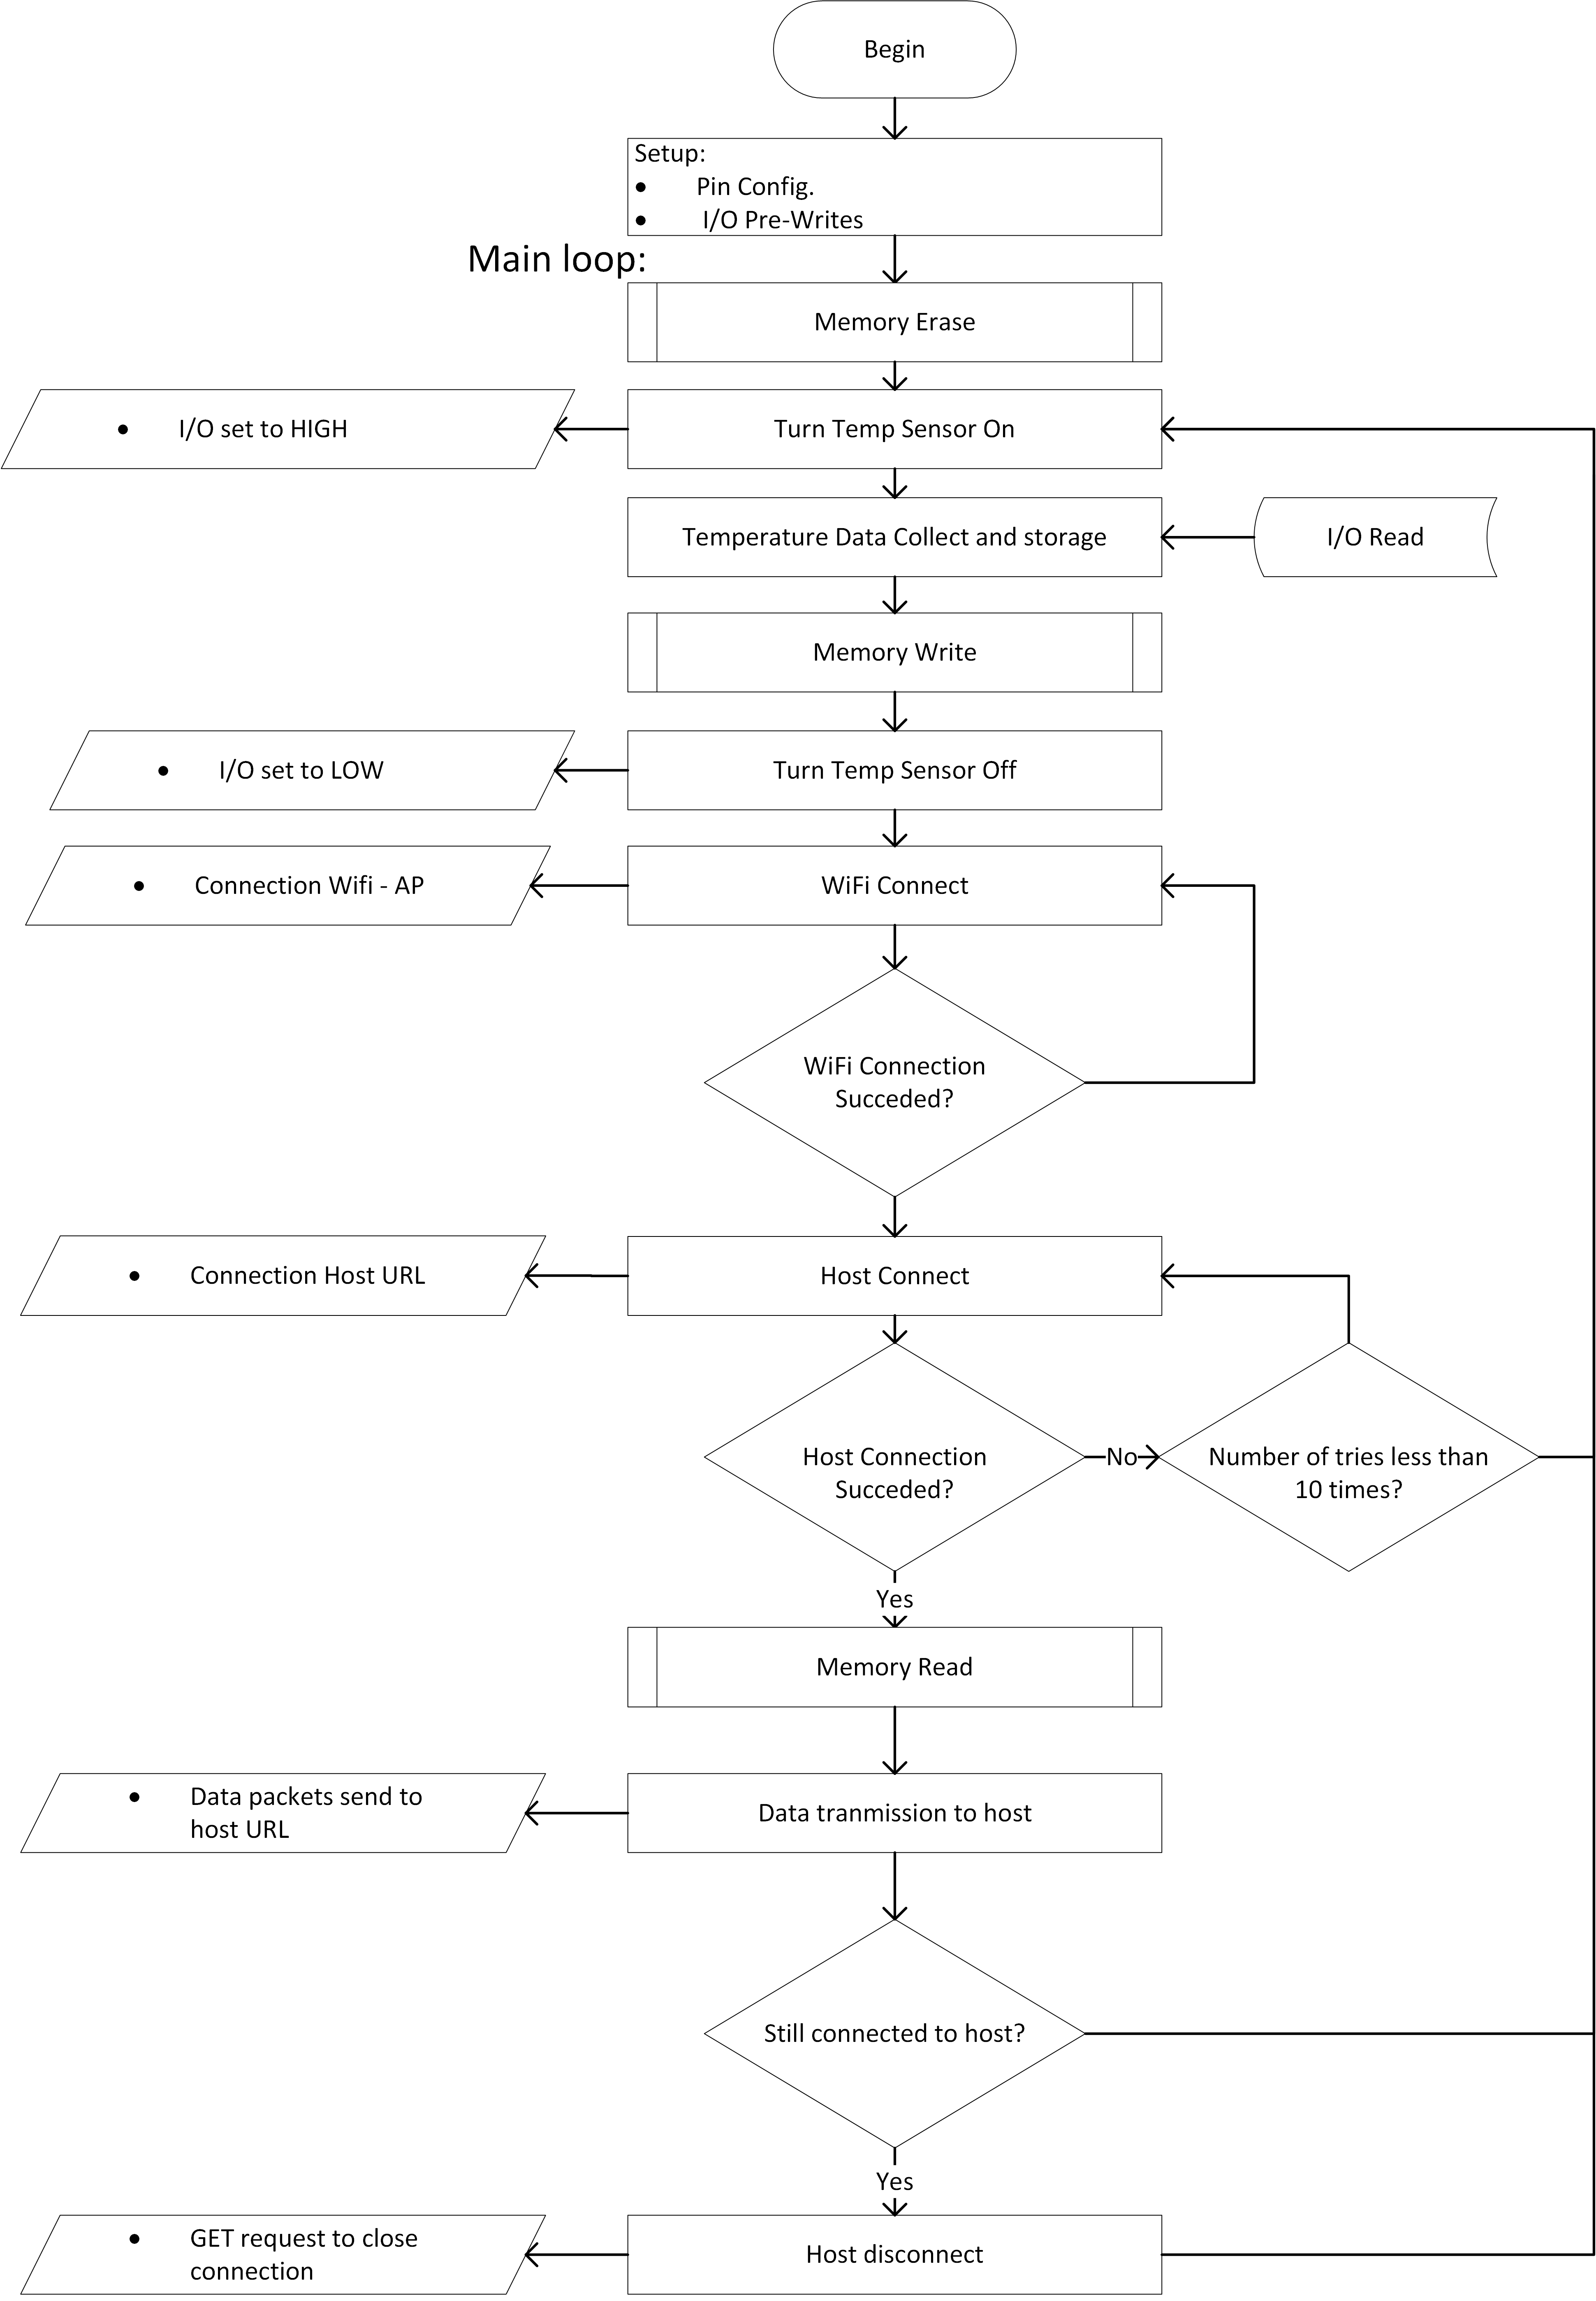
\includegraphics[scale = 0.9]{imagens/FA.png}
    \caption{\textbf{High level overview of the firmware}.}
    \label{02fig:FA}
\end{figure}



\subsection{Features and Algorithms}\label{04Sub:FeaturesAndAlgorithms}

In order to stabilize the instantaneous temperature readings, an Moving Average Filter Algorithm was implemented in the 
project. This algorithm takes a series of temperature measurements and calculates their average over a specified window of 
time or number of samples. By smoothing out variations and fluctuations in the temperature data, the Moving Average Filter 
Algorithm helps to provide a more stable and reliable temperature reading. \\ 

Additionally, as part of a possible future implementation, a general 3-byte array generator algorithm was implemented. This 
algorithm takes a long variable in the form of six nibbles "0xXYZWTR" as input. It then extracts and organizes the individual 
nibbles of the long variable into a 3-byte array. This allows for efficient storage and manipulation of the long variable in 
byte-based operations. The 3-byte array representation offers flexibility for future use, such as data transmission, storage, 
or further processing, depending on the project's requirements. \\ 

In addition to the mentioned components, the project also incorporates subroutines for Data Memory operations, 
including Write, Read, and Erase functionalities. These subroutines enable the program to interact with the Data Memory 
module connected to the ESP8266. The Write subroutine facilitates the storage of data, such as temperature readings or other 
relevant information, into the Data Memory. The Read subroutine allows retrieving data from the Data Memory, enabling access 
to previously stored information. Lastly, the Erase subroutine provides a mechanism to clear or reset the Data Memory, erasing 
any existing data stored within it. By implementing these subroutines, the project gains the capability to effectively manage 
and manipulate data in the Data Memory module, facilitating data logging, analysis, or further processing as required.




\subsection{Interfaces and Protocols}\label{04Sub: InterfacesAndProtocols}

In the project, a routine for SPI communication using bit banging was implemented. This approach allows direct control over 
the individual signal lines involved in the SPI protocol. The SPI protocol is widely used for communication between 
microcontrollers and peripheral devices such as the data memory chip in this case. The implemented routine operates on Mode 0, 
which is accepted by the data memory chip. Mode 0 means that the clock signal is idle low, and data is sampled on the leading 
edge of the clock signal. \\ 

The SPI communication routine has a clock period of 6 microseconds (6$\mu s$), resulting in a frequency of approximately 
166,666 kHz. This frequency falls within the acceptable range supported by the memory IC, ensuring reliable and efficient data 
transfer. By utilizing bit banging and adhering to the Mode 0 protocol with an appropriate clock frequency, the implemented 
routine enables effective communication between the ESP8266 and the data memory chip, facilitating data read/write operations 
and supporting the overall functionality of the project. \\ 












%%%%%%%%%%%%%    END   %%%%%%%%%%%%%
%%%%%%%%      Firmware      %%%%%%%%
%%%%%%%%%%%%%%%%%%%%%%%%%%%%%%%%%%%%